%% Section1-Abstract.tex
%% 绪论

\chapter{绪论}
\section{基本概念}
\begin{itemize*}
    \item \textbf{激光成像}:Laser Imaging, LI.
    \item \textbf{激光遥感}:Laser Remote Sensing, LRS.
    \item \textbf{激光雷达}:Light Detection And Ranging, LiDAR.
    \item \textbf{机载激光地形测绘}:Airborne Laser Terrain Mapping, ALTM.
    \item \textbf{机载激光制图}:Airborne Laser Mapping, ALM.
    \item \textbf{机载激光扫描}:Airborne Laser Scanning, ALS.
    \item \textbf{机载激光测高}:Airborne laser altimetry, ALA.
    \item \textbf{激光测高}:Laser Altimetry, LA.
    \item \textbf{机载激光扫描测高}:Airborne Laser Scanning Altimetry, ALSA.
    \item \textbf{空载光达、空载雷射扫描}:Light Detection And Ranging, LiDAR.
\end{itemize*}

\section{应用现状}
\begin{enumerate*}
	\item % 森林检测与管理
	\textbf{森林检测与管理}。LiDAR系统的最早商业应用领域之一。\\
	\textbf{传统技术}:以前是借助空中摄影和地面测量进行的。这些方法不仅费时费力,而且只能分析样点,结果还是推断的。\\
	\textbf{激光雷达的优势}:激光扫描法能克服这些缺点,通过激光扫描技术
	提取得完整的3D森林模型。在单个树木分析的基础上,可确定以下的参数:\begin{itemize*}
		\item 单个树高
		\item 一片林区的平均树高
		\item 一片林区的木材体积
		\item 一片林区的平均密度
		\item 每片林区的平均生长体积
	\end{itemize*} 
	此外LiDAR得到的DTM还可以来规划和改善森林运输道路,以及进行倾斜度分析,以便测定危险。
	\item % 构建数字城市模型
	\textbf{构建数字城市模型}
	在电信、无线通讯、法律实施和灾难管理等众多领域中都
	需要准确的数字城市模型(建筑物建模、城市规划、噪
	声模拟、无线网络规划)
	\item % 湿地、限制进入地区、危险区域
	\textbf{湿地、限制进入地区、危险区域}
	\begin{itemize}
		\item 密集的植被覆盖和没有可通行的道路。
		\item 传统的地面摄像测量技术很难对沼泽、野生动物保护区及森林保护区进行勘测。
		\item 危险地带的地貌特征获取。
	\end{itemize}
	\item \textbf{油气管道勘测}
	\item \textbf{洪水灾情预测}(洪水制图、灾害评估)获取流域的数字表面模型和数字高程模型。
	\item \textbf{海岸线监测与制图}
	\item \textbf{水深、海岸线、侵蚀状况监测}
	\item \textbf{电力线监测}
	\item \textbf{股文物保护}
	\item \textbf{真正射影像的制作}
\end{enumerate*}

\section{LiDAR技术特点}
\begin{enumerate*}
	\item 无需光照条件或专门的太阳高度角。
	\item 可在白天、夜晚或相当恶劣的条件下(大雾)作业,全天时全天候获取地面三维数据。
	\item 能部分“穿透”植被,同时测量地面和非地面层。
	\item 很少需要进入测量现场,不需要大量的地面控制点。
	\item 能快速获取数据,24小时内可提取测区的DEM数据。
	\item 精度较高。
	\item 能够接受无穷次回波。
	\item 可在地面反射率比较低的区域工作,例如反射率只有约5\%的地面。
	\item 集成RS和GPS技术,数据可直接作为GIS的数据源,有利于提高地理数据的自动化,加快处理速度。
	\item 一个飞行日内可采集高达200 GB的数据。
	\item 高速度、高性能、高精度、长距离的航空测量设备。
	\item 全数字化,可直接产生三维坐标$ (X,Y,Z) $,无需其他额外步骤。
	\item 数据密集。基于固定翼机载平台采集时,典型的激光光斑中心间距为0.5 m左右。
	\item 精度:针对地物建模应用情形,典型精度达15 cm。
	\item 机载平台:便于操作,易于快速获取地表数据。
	\item 宽视场角:最大可以达到$ 75^{\circ} $的视场角。如果部分视场角范围没有被用到,可以用于飞机倾角稳
	定补偿。
\end{enumerate*}

\section{激光成像技术}
\subsection{激光}
\paragraph{地位}激光是20世纪以来,继原子能、计算机、半导体之后,人类的又一重大发明,被称为“最快的刀”、“最准的尺”、“最亮的光” 。
\paragraph{激光的亮度}约为太阳光的100亿倍。
\paragraph{激光的特点} \begin{itemize*}
	\item 单色性、方向性、相干性
	\item 具有很高的单光子辐射能量
	\item 在大气传输中很少发生绕射
\end{itemize*}
\paragraph{激光设备}1960年发明红宝石激光器,主要在军事上得到了应用。\begin{itemize*}
	\item \textbf{激光测距仪}:美国1969年测地月距离。
	\item \textbf{激光致盲器}:1982年英阿马岛战争投入实战。
	\item \textbf{激光制导器}:1991年海湾战争,精度高、抗干扰能力强。
	\item \textbf{激光告警设备、激光干扰设备}等电子战装备。
\end{itemize*}
\paragraph{激光的应用}\begin{itemize*}
	\item \textbf{自然科学}
	\item \textbf{加工领域}
	\item \textbf{信息处理}
	\item \textbf{激光通信}
	\item \textbf{医学领域}
	\item \textbf{测绘领域}
	\item \textbf{环境检测}:弥补了微波在绕射和不能探测目标生化特性的不足,有了更加广泛的应用范围。 \begin{itemize*}
		\item 大气成分探测(气溶胶探测)
		\item 污染探测大气和海洋基本参数,如:海水深度、温度等探测。
		\item 绿色植物探测
	\end{itemize*}
\end{itemize*}
\paragraph{微波雷达的局限性}\begin{itemize*}
	\item 其波长较长,相应能量子的能量很小。
	\item 一般不足以与目标发生生化作用,无法探测目标的生化特性。
	\item 在传播过程中,遇到尺寸小于波长的物体时,更易于发生衍射。
\end{itemize*}
\subsection{激光雷达与激光成像雷达}
\paragraph{激光雷达的光源类型}\begin{itemize*}
	\item 可见光波段\ce{He}-\ce{Ne}和\ce{Ar}激光器
	\item 短波红外波段Nd:YAG激光器。最成熟的激光器。
	\item 长红外波段的\ce{CO2}激光器。正在研制的大多是\ce{CO2}激光器,体积大,价格比较高。
	\item 二极管泵浦固体激光雷达(DPL),20世纪80年代后期。是发展重点。\\
	\textbf{DPL的优点}:\begin{itemize*}
		\item 无需制冷
		\item 不像红外热成像系统容易受环境影响
		\item 对人眼安全,大气消光比低
		\item 可采用光纤光路和集成光学技术
		\item 结构小型化,体积小,制作成本低
		\item 具有高稳频、高功率、高效率和高光束质量等优点
		\item 可距离成像和强度成像
	\end{itemize*}
	\textbf{DPL与其他激光器的比较}:\begin{itemize*}
		\item \textbf{与Nd:YAG激光器相比}:后者只能测距和测角,不能测速,成像困难,大气传输性较差。
		\item \textbf{与\ce{CO2}激光器相比}:相干性好,寿命长,可靠性强。
	\end{itemize*}
	\textbf{DPL的应用}\begin{itemize*}
		\item 军事的应用
		\item 大气测污、风场测量、环境监测
	\end{itemize*}
\end{itemize*}
\paragraph{激光成像雷达的基本结构} 如图\ref{fig:激光成像雷达的基本结构}所示。
\begin{figure}[htbp]
	\centering
	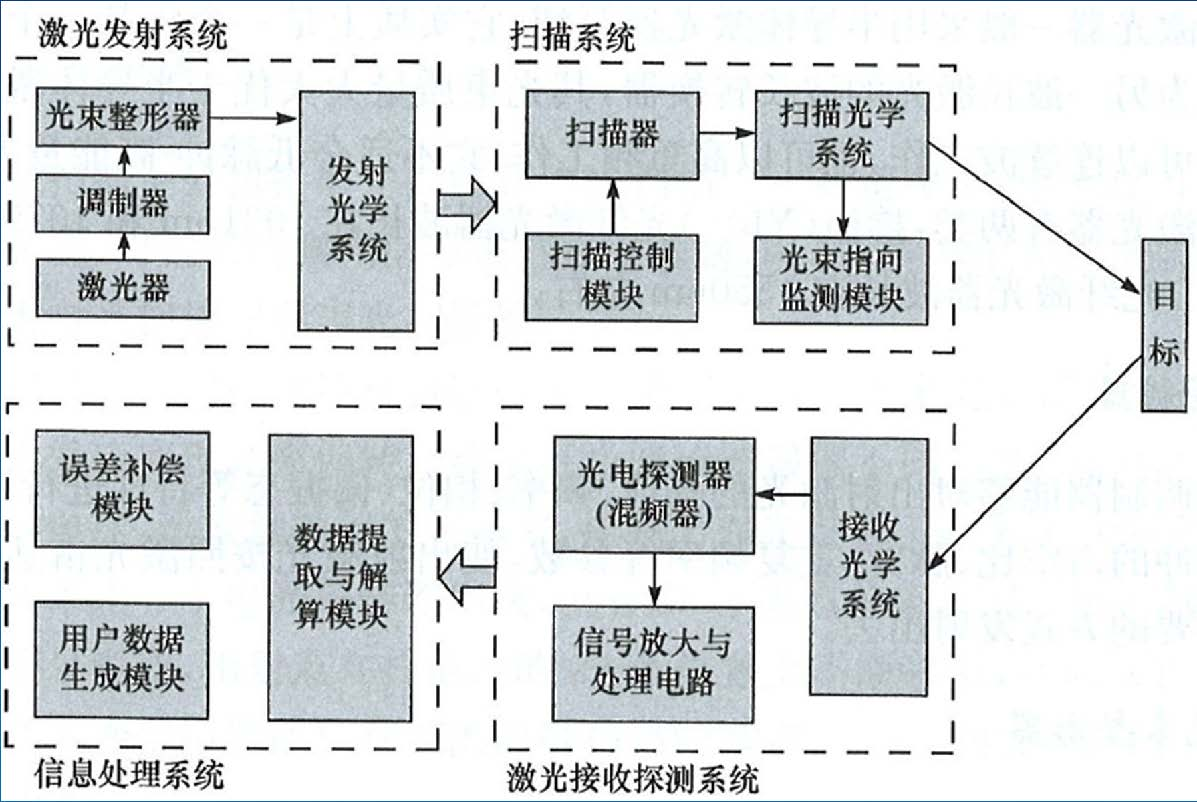
\includegraphics[width=0.7\linewidth]{figure/Chapter1/激光成像雷达的基本结构.jpg}
	\caption{激光成像雷达的基本结构}
	\label{fig:激光成像雷达的基本结构}
\end{figure}
\paragraph{激光雷达的关键技术} 下列四项技术中,前三项属于硬件技术,均已得到不同程度的解决;第四项技术属于软件技术,目前成为最关键的技术。
\begin{enumerate*}
	\item \textbf{激光发射器}:高功率和高波束质量的辐射源
	\begin{enumerate*}
		\item \textbf{气体激光器}。\\
		\textbf{特点}:\begin{itemize*}
			\item 典型的气体激光器为\ce{CO2}
			\item 最早用于激光雷达的激光器之一
			\item 工作波长为10.6 $ \symrm{\mu m} $,处于大气窗口。
			\item 至今仍广泛用于激光雷达
		\end{itemize*}
		\textbf{优点}:\begin{itemize*}
			\item 大气传输性能好,效率高。
			\item \ce{CO2}激光雷达易于实现高灵敏度外差探测和三维成像,信息处理技术成熟。
		\end{itemize*}
		\textbf{缺点}:\begin{itemize*}
			\item 尺寸比较大
			\item 需要低温制冷
		\end{itemize*}
	\end{enumerate*}
	\item \textbf{成像探测器}:高灵敏度接收技术
	\item \textbf{扫描系统}:高性能二维扫描技术
	\item \textbf{数据处理技术}:图像处理及目标识别算法
\end{enumerate*}